\begin{center}
	\begin{tikzpicture}[x=1cm,y=1cm]
	%\pgfresetboundingbox
	\draw[use as bounding box, anchor = north west,draw=none] (-5.5,-3.25) rectangle (5.5,3.25);
	\clip (-5.5,-3.25) rectangle (5.5,3.25);
	\node[anchor =north west] (text) at (-5.25,3.25){\begin{minipage}{10.0cm}
	Warning: this talk contains some \textit{light} mathematics.\\$ $\\
	\visible<3->{
	Some useful notation:\\$ $\\ 
	\begin{tabular}{p{3cm}p{6cm}}
	\hline $X$& training data, as rows\\
	$x^{*} $& one new molecule/systems\\
	$y,\hat{y}$ & property(energy?), predicted value\\
	$\mathcal{L}=\left\Vert y - \hat{y}\right\Vert_2^2 $ & loss function\\
	$W,w$ & model parameters\\
	$\hat{y}=f(x,W)$ & our model\\\hline 
	\end{tabular}
	
	}
	\end{minipage}};
	\visible<2>{\node (figure) at (0,-0.75){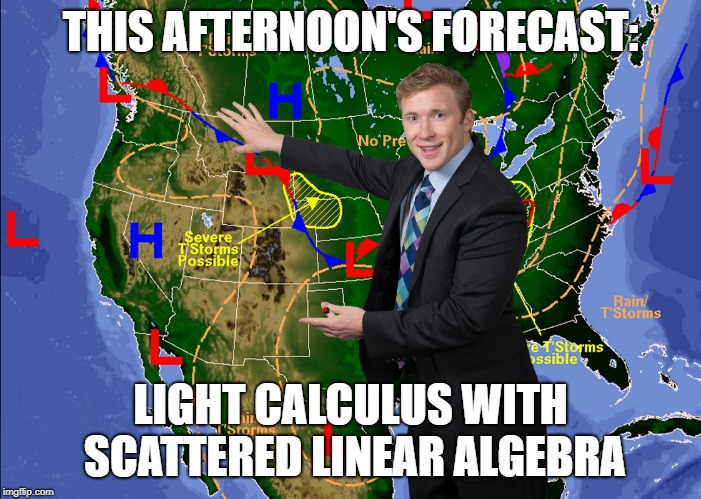
\includegraphics[width=6.5cm]{images-top/weather.jpg}};}
\end{tikzpicture}
\end{center}
